\documentclass{article} % For LaTeX2e
\usepackage{cos424,times}
\usepackage{hyperref}
\usepackage{url}
\usepackage{graphicx}
\usepackage{amsmath}
%\usepackage{natbib}
\usepackage{multirow}
\usepackage{bm,bbm}
\usepackage{amssymb}
\usepackage{float}
\usepackage{subcaption}
\title{Fragile Families Challenge}

\author{
Andrew Or\\
Department of Computer Science\\
Princeton University\\
\texttt{andrewor@cs.princeton.edu} \\
\And
Thomas Shaffner \\
Department of Computer Science \\
Princeton University \\
\texttt{tfs3@cs.princeton.edu} \\
}

\newcommand{\fix}{\marginpar{FIX}}
\newcommand{\new}{\marginpar{NEW}}

\begin{document}

\maketitle

\begin{abstract}

This paper describes our submission to the Fragile Families Challenge \cite{ffc}, an effort that applies techniques in predictive modeling and causal inference to interviews conducted with disadvantaged families. The goal of the project is to improve the lives of children in these families by identifying underlying patterns in the answers given by the families. In this work, we use regression and classification methods to predict the values of six key attributes: GPA, grit, material hardship, eviction, layoff, and job training. Because of the abundance of invalid entries in the data, feature selection plays a crucial role in our effort.

\end{abstract}
\section{Introduction}
\label{sec:intro}

The Fragile Families and Child Wellbeing Study (FFCWS) \cite{ffcws} is an academic collaboration that follows around 5,000 urban families in the United States and collects information about how their social environments change over time. Interviews were first conducted shortly after the birth of the family's child between 1998 and 2000, then were conducted again when the child was age one, three, five, nine, and fifteen. Because of the goal is to understand the difficulty face by disadvantaged families, non-marital births are overrepresented (roughly three-quarters of all births) in the study.

The data collected in this study has been used by academic papers published in many journals since then \cite{ffc_publications}. Insights derived from this data are shared with policy makers through the Future of Children \cite{foc}, a collaboration between the Woodrow Wilson School of Public and International Affairs at Princeton University and the Brookings Institution.

The Fragile Families Challenge is an open challenge for data scientists to apply machine learning and statistical methods to the data collected in this study. The challenge aims to use ensemble methods on the best models submitted to discover factors correlated with children beating the odds.

In this paper, we propose our solution to the Fragile Families Challenge. We modeled continuous labels and binary labels separately, using regression methods for the former and classification methods for the latter. The regression methods we evaluated are:

\begin{enumerate}
\item Linear Regression with Lasso Regularization (LRL)
\item Support Vector Regression (SVR)
\item Random Forest Regression (RFR)
\end{enumerate}
and the classifiers we evaluated are:
\begin{enumerate}
\item Bernoulli Naive Bayes Classifier (BNB)
\item Multinomial Naive Bayes Classifier (MNB)
\item K-Nearest Neighbors Classifier (KNN)
\item Random Forest Classifier (RFC)
\item Gradient Boosting Classifier (GBC)
\end{enumerate}

We used the \texttt{scikit-learn} implementation of all of the above regression and classification methods. The main metrics we used in our evaluation are the coefficient of determination (also known as the $R^2$ score) for continuous labels and accuracy for binary labels. In both cases, we found that Random Forest performs the best. We used k-fold cross validation to tune the hyperparameters of these models to yield better generalization error. To account for the abundance of missing or invalid values in the dataset, we experimented with various feature selection and imputation techniques, such as $\chi^2$ feature reduction and filling null values with the mean and mode of the column.

All source code is available on Github at \cite{myrepo}.

\section{Dataset}
\label{sec:dataset}

The background data is primarily composed of answers collected from interviews with the families over the years. These are the features used to train our models. Each row uniquely identifies a child and each column is either an ID of some form or an interview answer. In this dataset, there are 4242 rows and 12945 columns.

The label data consists of six labels we wish to predict based on the features in the background data. These labels are derived from a final interview with the child when he or she is age 15. The six labels are: GPA, grit, material hardship, eviction, layoff and job training. The first three are continuous labels while the latter three are binary labels. There are 2121 rows in the label data, exactly half the number of rows in the background data. The goal is to predict the six labels for the 2121 missing rows using the background data.

Unfortunately, both sets of data were filled with invalid entries, such as N/A, string values, and specific negative values in the background case. The background data has 12945 columns, of which 3090 columns have null values (23.9\%), 147 columns have string values (1.14\%), and 10459 have negative values (80.8\%). Only 42 columns have neither null nor negative values, but up to 14 of these refer to some sort of ID and thus are not appropriate for being used as features. Thus, aggressive feature selection and imputation strategies must be used to yield a good fit, as we discuss in the next section. 

Similarly, the label data is filled with null values. In particular, out of the 2121 rows, 956 GPA values (45.1\%), 703 grit values (33.1\%), 662 material hardship values (31.2\%), 662 eviction values (31.2\%), 844 layoff values (39.8\%), and 660 job training values (31.1\%) were null. Across all labels, as many as 655 rows were all nulls (30.9\%). The null label values were not considered in our evaluation.

\section{Data processing}
\label{sec:datapreprocessing}

We used several imputation and feature selection methods to prepare the background data before training classification and regression models. Here we describe the individual strategies used for imputation and feature selection, and the schemes produced by combinations of these techniques.

\subsection{Imputation}
\label{sec:imputation}

Because such a large fraction of the background dataset consists of invalid entries, we tested strategies to impute the underlying true values for these entries. In particular, we experimented with the following:

\begin{itemize}
\item \textbf{Simple imputation:} Replace N/A with mode, negative values with $1$.
\item \textbf{Averaging imputation:} Replace N/A with mode, negative values with mode or mean of valid values of the feature. Mode is used if the feature type is integer and mean is used if the feature type is float.
\end{itemize}

Imputation does not make sense for string columns so we simply discarded these columns instead, as we discuss next.

\subsection{Feature selection}
\label{sec:featureselection}

We used several methods of varying complexity to remove features from the background dataset.

\begin{itemize}
  \item \textbf{String removal:} Remove features that contain at least one string
  \item \textbf{Null removal:} Remove features that contain at least one N/A value
  \item \textbf{Negative removal (r):} Remove features whose fraction of negative values is $\geq \texttt{r}$
  \item \textbf{Chi-squared (k):} Select $k$ features with lowest $\chi^2$ score
\end{itemize}

\subsection{Evaluated schemes}
\label{sec:evaluatedschemes}

We evaluated five schemes composed of combinations of the imputation and feature selection strategies listed above:

\begin{itemize}
\item \textbf{Baseline:} simple imputation + string removal = 12798 features
\item \textbf{No null:} simple imputation + string removal + null removal = 9844 features
\item \textbf{Data type dependent imputation:} average imputation + string removal + null removal = 9844 features
\item \textbf{Negative proportions (r):} simple imputation + string removal + null removal + negative removal ($r$)
  \begin{itemize}
    \item{913 features for $r = 0.25$}
    \item{2718 features for $r = 0.5$}
    \item{3807 features for $r = 0.75$}
  \end{itemize}
\item \textbf{Chi-squared feature reduction:} simple imputation + string removal + null removal + chi-squared ($k$) = $k$ features
\end{itemize}

In our evaluation, we found that the \textit{no null} scheme yielded the best results for both continuous and binary labels. We decided to experiment with \textit{data type dependent imputation} because we found simply replacing all negative values with $1$ arbitrary. We also believed (incorrectly) that removing features with negative values in the \textit{negative proportions} scheme would help because negative values indicate invalid or missing answers.

Similarly, \textit{chi-squared feature reduction} consistently led to worse results. In an effort to understand why this is the case, we confirmed that non-indicative features such as \texttt{challengeID} and \texttt{mothid1} (mother ID) had high $\chi^2$ scores, while hundreds of features had a $\chi^2$ score of 0. Oddly, even setting $k = 99.5\%$ of the total number of features led to a significant drop in accuracy for the binary case. 
As such, we did not consider Chi-squared feature reduction further in our project.

\section{Classification and Regression}
\label{sec:regression}

We tested several classification and regression methods (detailed in Section~\ref{sec:intro}), but ultimately used random forest methods for both classification and regression tasks. Here we discuss in more detail the specifics of random forest regression.

Random forest regression methods are used to combine multiple regression trees. The random forest regression algorithm draws uniformly at random $m$ subsets of the training data. The algorithm then trains a regression tree on each of the subsets.

\begin{figure}[H]
  \centering
  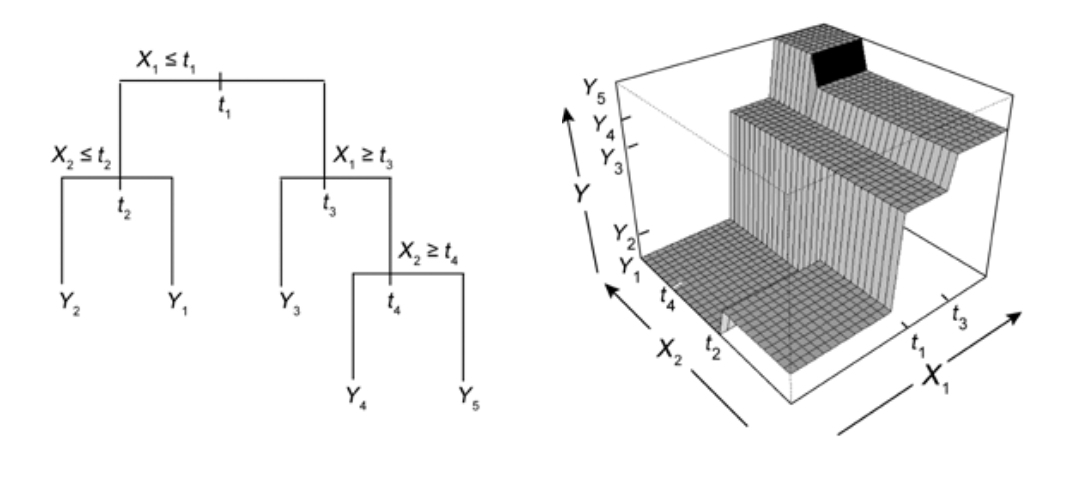
\includegraphics[width=0.7\textwidth]{rf.png}
  \caption{An example regression tree, borrowed from \cite{rffig}}
  \label{fig:regtree}
\end{figure}

In the same manner as decision trees, regression trees split samples at branch points based on feature values (see Figure~\ref{fig:regtree}). Given training samples $x_i$ and (continuous) training response variables $y_i$, regression trees are built in the following manner.

\begin{enumerate}
  \item Select the optimal feature $f$ and value $v_f$ for branching by minimizing $RSS$
  \item Partition samples into $L = \{i | x_{if} \leq v_f\}$ and $R = \{j | x_{jf} > v_f\}$
  \item Recurse on the subsets $L$ and $R$ of input data
\end{enumerate}

with $RSS$ defined as

\begin{align*}
  RSS &= \sum_{i \in L} (y_i - y_L^*)^2 + \sum_{j \in R} (y_j - y_R^*)^2
\end{align*}

and where $y_L^* = \frac{1}{\lvert L \rvert} \sum_{i \in L} y_i $ is the mean of all response variables corresponding to samples in the left subtree of the branch point, and $y_R^* = \frac{1}{\lvert R \rvert} \sum_{j \in R} y_j$ is the mean of all response variables corresponding to samples in the righthand subtree.

Given a new sample $x$, a single regression tree determines which leaf represents $x$ and assigns to $x$ the predicted $y$ value of the mean of all response values represented by that leaf. Random forest regressors, given a new sample $x$, return as a prediction the average of the responses of each regression tree.

\section{Evaluation}
\label{sec:evaluation}

\subsection{Hyperparameter tuning}
\label{sec:hyperparametertuning}

We used cross-validation to tune hyperparameters for the random forest regressors and classifiers used to predict response variables. We chose to tune $\texttt{n\textunderscore estimators}$ representing the number of regression trees trained, $\texttt{max\textunderscore features}$ representing the portion of all features to examine while generating splits, and $\texttt{min\textunderscore samples\textunderscore split}$ representing the minimum number of samples in a node before it is allowed to split. Each of these hyperparameters provides a method avoid overfitting, as they each place restrictions on the growth of decision and regression trees. Specifically, we used the $\texttt{GridSearchCV}$ and $\texttt{RandomSearchCV}$ methods from the $\texttt{scikit-learn}$ Python package. Figure~\ref{fig:params} denotes the values which we tested for each hyperparameter in both the continuous regression (Figure~\ref{fig:contparams}) and boolean classification (Figure~\ref{fig:boolparams}) cases.

\begin{figure}[H]
  \centering
  \hfill
  \begin{subfigure}[b]{0.35\textwidth}
    \begin{align*}
      &\texttt{n\textunderscore estimators}:~50,~75,~100\\
      &\texttt{max\textunderscore features}:~0.75,~1.0\\
      &\texttt{min\textunderscore samples\textunderscore split}:~10,~25,~50
    \end{align*}
    \caption{Options for continuous regression}
    \label{fig:contparams}
  \end{subfigure}
  \hfill
  \begin{subfigure}[b]{0.35\textwidth}
    \begin{align*}
      &\texttt{n\textunderscore estimators}:~50,~100\\
      &\texttt{max\textunderscore features}:~0.75,~1.0\\
      &\texttt{min\textunderscore samples\textunderscore split}:~10,~25
    \end{align*}
    \caption{Options for boolean classification}
    \label{fig:boolparams}
  \end{subfigure}
  \caption{Hyperparameter options}
  \label{fig:params}
  \hfill
\end{figure}

The results of this cross-validation hyperparameter tuning are shown in Table~\ref{tab:optimalparams}. Note that different values are optimal for different labels.

\begin{table}[H]
  \centering
  \fontsize{9}{11}\selectfont
  \begin{tabular}{| c | c | c | c | c | c | c | c |}
    \hline
    ~ & \texttt{gpa} & \texttt{grit} & \texttt{materialHardship} & \texttt{eviction} & \texttt{layoff} & \texttt{jobTraining} \\ \hline
    \texttt{n\textunderscore estimators} & 100 & 75 & 100 & 50 & 50 & 50 \\
    \texttt{max\textunderscore features} & 1.0 & 0.75 & 0.75 & 0.75 & 1.0 & 0.75 \\
    \texttt{min\textunderscore samples\textunderscore split} & 50 & 50 & 10 & 25 & 25 & 25 \\
    \hline
  \end{tabular}
  \caption{Optimal hyperparameters for each label}
  \label{tab:optimalparams}
\end{table}

\subsection{Results}
\label{sec:results}

We evaluated continuous variable predictions using the $R^2$ coefficient of determination defined as. Given $n$ true continuous labels $y_i$, let $\bar{y} = \frac{1}{n}\sum_{i=1}^n y_i$ be the mean of all labels. Let the predicted labels be denoted $\hat{y}_i$. The $R^2$ coefficient of determination is then defined as

\begin{align*}
  R^2 &= 1 - \frac{\sum_{i=1}^n (y_i - \hat{y}_i)^2}{\sum_{i=1}^n (y_i - \bar{y})^2}
\end{align*}

In addition to accuracy, we evaluated boolean variable predictions with precision, recall, and F1 scores. The F1 score is the harmonic mean of precision and recall, and is there greater when both precision and recall are greater.

\begin{table}[H]
  \begin{minipage}{0.30\textwidth}
    \centering
    \begin{tabular}{| c | c | c | c |}
      \hline
      ~ & LRL & SVR & RFR \\ \hline
      $R^2$ & 0.063 & 0.123 & 0.157 \\
      \hline
    \end{tabular}
    \caption{Evaluation of different models for continuous regression of \texttt{gpa}}
    \label{tab:contresults}
  \end{minipage}%
  \hfill
  \begin{minipage}{0.60\textwidth}
    \centering
    \begin{tabular}{| c | c | c | c | c | c |}
      \hline
      ~ & BNB & MNB & KNN & RFC & GBC \\ \hline
      Accuracy & 0.761 & 0.584 & 0.725 & 0.765 & 0.679 \\
      Precision & 0.040 & 0.244 & 0.253 & 0.000 & 0.204 \\
      Recall & 0.003 & 0.362 & 0.085 & 0.000 & 0.130 \\
      F1 & 0.005 & 0.285 & 0.126 & 0.000 & 0.157 \\
      \hline
    \end{tabular}
    \caption{Evaluation of different models for binary classification of \texttt{jobTraining}}
    \label{tab:boolresults}
  \end{minipage}
\end{table}

We found that random forests performed best for both $R^2$ and Accuracy. This dataset is likely not linearly separable under reasonable imputation and feature selection schemes. Therefore, we expect that random forest regression would perform better than either support vector regression or linear regression. Also, because there are significantly more False values than True values across the boolean variables, all predictors are heavily skewed towards predicting False. This leads the random forest classifier to predict all False scores, which is why we observe precision, recall, and F1 scores of 0 for RFC

\subsection{Beating the odds}
\label{sec:beatingtheodds}

We were interested in determining which children ended the study with better metrics than we would predict with our model. Higher values of gpa and grit are considered better, while a lower value of material hardship is considered better. Therefore, we consider samples with higher gpa, higher grit, or lower material hardship than our predictions to have ``beaten the odds''. Similarly, we consider any sample that disagrees with our prediction and is False for eviction, False for layoff, or True for job training to have beaten the odds.

For each continuous variable, we ranked the samples by the margin to which they beat their prediction. We hoped to see high overlap in the tops of each of these ranked list. However, we found that there were no samples common to the top $100$ positions in all lists, and there were only ten samples common to the top $250$ samples in all lists.

Because our best-performing model predicts False for all boolean variables for all samples, we observe no samples beating the odds for eviction or layoff, while every subject that has received job training has beaten the odds according to our model and definition.

We hypothesize that we do not observe subjects who consistently beat the odds by a high margin because we train models for each variable independently using different hyperparameters. For future work, it would be interesting to train multiple labels together to see if larger overlaps occur between the subjects who beat the odds by the highest margins for each label.

\section{Conclusion}
\label{sec:conclusion}

Due to the nature of the background data provided, we find that random forest methods perform best for both classification and regression problems. However, the fact that boolean training data is heavily skewed towards responses of ``False'' leads our random forest classification model to predict False for every test sample. Furthermore, there are many invalid responses throughout the background dataset. We hypothesize that this data sparsity causes standard feature selection techniques like chi-squared analysis to produce worse results.

We also identified rankings subjects who beat the odds by the highest margin for continuous variables. Though there is little overlap between the tops of these rankings, we propose training a single predictive model on a combination of labels in order to better determine whether any subjects consistently beat the odds by high margins.

\begin{thebibliography}{}

\bibitem{myrepo}
https://github.com/andrewor14/ffc

\bibitem{ffc}
Fragile Families Challenge: http://www.fragilefamilieschallenge.org/

\bibitem{ffcws}
Fragile Families and Child Wellbeing Study: http://www.fragilefamilies.princeton.edu/

\bibitem{ffc_publications}
Fragile Families publications: http://crcw.princeton.edu/publications/publications.asp

\bibitem{foc}
Future of Children: http://www.futureofchildren.org/

\bibitem{randomforest}
Breiman, Leo. "Random forests." Machine learning 45.1 (2001): 5-32.

\bibitem{confidenceweight}
Dredze, Mark, Koby Crammer, and Fernando Pereira. "Confidence-weighted linear classification." Proceedings of the 25th international conference on Machine learning. ACM, 2008.

\bibitem{randomsubspace}
Ho, Tin Kam. "The random subspace method for constructing decision forests." IEEE transactions on pattern analysis and machine intelligence 20.8 (1998): 832-844.

\bibitem{individuallabel}
Kotzias, Dimitrios, et al. "From group to individual labels using deep features." Proceedings of the 21th ACM SIGKDD International Conference on Knowledge Discovery and Data Mining. ACM, 2015.

\bibitem{textbook}
Murphy, Kevin P. Machine learning: a probabilistic perspective. MIT press, 2012.

\bibitem{scikitlearn}
Pedregosa, Fabian, et al. "Scikit-learn: Machine learning in Python." Journal of Machine Learning Research 12.Oct (2011): 2825-2830.

\bibitem{id3}
Quinlan, J. Ross. "Induction of decision trees." Machine learning 1.1 (1986): 81-106.

\bibitem{rffig}
Elith, Jane, John R. Leathwick, and Trevor Hastie. "A working guide to boosted regression trees." Journal of Animal Ecology 77.4 (2008): 802-813.
 
\end{thebibliography}

\end{document}

